\section{Filter Parameters}
Given the project specifications, it is possible to draw the \textbf{Data Flow Diagram} as shown in \autoref{lab1:fig:iir-dfd}.
\begin{figure}[htbp]
	\center
	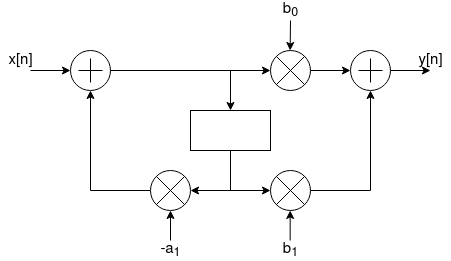
\includegraphics[width=0.65\textwidth]{chapter1/images/iir-dfd.png}
	\caption{Target filter data flow diagram}
	\label{lab1:fig:iir-dfd}
\end{figure}

This DFD implements the Direct Form II of an IIR filterand, in this specific case, implements the following equations:
\begin{align}\label{eqn:iir2}
	w[n] &= x[n] - a_1 w[n-1] \\
	y[n] &= b_0 w[n] + b_1 w[n-1]
\end{align}
It is thus necessary to determine the values of the $a$ and $b$ parameters. Thanks to the provided Matlab script \texttt{myiir\_design.m}, the derived results are:
\begin{align}
    a &= [-21] \\
    b &= [53,\ 53]
\end{align}
